% Research draft using the unmodified official CVPR 2027 author-kit style.
% Replace the author field before sharing as an authored manuscript.
% Use [review] instead of [pagenumbers] only after anonymizing the draft.
\documentclass[10pt,twocolumn,letterpaper]{article}
\usepackage[pagenumbers]{cvpr}
\usepackage{amsmath,amssymb,booktabs,graphicx,microtype}
\usepackage{colortbl}
\definecolor{ourrow}{RGB}{230,242,250}
\usepackage[breaklinks,colorlinks,allcolors=cvprblue]{hyperref}
\definecolor{cvprblue}{rgb}{0.21,0.49,0.74}
\def\confName{CVPR}
\def\confYear{2027}
\newcommand{\sg}{\operatorname{sg}}
\newcommand{\CE}{\operatorname{CE}}
\newcommand{\KL}{\operatorname{KL}}
\newcommand{\NCE}{\mathcal{L}_{\mathrm{NCE}}}
\newcommand{\JS}{\mathcal{L}_{\mathrm{JS}}}
\title{Adaptive Mixing of Stochastic Augmentation Chains\\
for Corruption-Robust Continual Learning}
\author{Research draft\\Author information to be supplied}
\begin{document}
\maketitle

\begin{abstract}
Learning representations that remain useful under unseen test-time corruptions
requires meaningful training variation. Yet the space of augmentation chains
grows combinatorially with operation choices and depth, making exhaustive
coverage computationally impractical. We investigate whether a learned mixer
can make better use of a limited set of randomly sampled chains in continual
learning. Building on a MetaMix-inspired setup, our chain-aware mixer uses
candidate feature and prediction changes together with temporal learner context
to adapt the weights of stochastic AugMix chains. The original-image weight
is fixed at one half to retain a transformed contribution. Classifier
representation learning and mixer adaptation use independently chosen
consistency objectives; these are training surrogates, not direct measurements
of unseen robustness. Across eight Split-CIFAR-10 experiments with DER++ replay,
chain-aware InfoNCE/JS achieves \textbf{56.22\% clean class-IL accuracy} and
\textbf{47.17\% on CIFAR-10-C}, improving on our guided mixer with the same
objectives by \textbf{7.96 and 8.62 percentage points}. This is the best clean
and second-best corrupted accuracy among the evaluated configurations; random
InfoNCE remains strongest on corruptions at 48.27\%. Matching both chain-aware
objectives performs worse. These single-seed findings provide qualified evidence
for adaptive mixing, while leaving candidate-conditioning effects and
compute--accuracy efficiency unestablished.
\end{abstract}

\section{Introduction}
We seek representations that support accurate classification under test-time
corruptions absent from training. In continual learning, this goal is coupled
with retaining knowledge as new tasks arrive: both the data available to the
learner and its representation evolve. Replay preserves access to earlier
examples, while augmentation exposes the learner to input variation. Our focus
is how to use a limited number of augmentation candidates to support robust
representation learning throughout this process.

The augmentation space is much larger than a short list of operations.
Different operation choices, orders, chain depths, and severity settings produce
a combinatorial family of compositions. Exhaustively training over this family
becomes computationally impractical as these choices grow; nor would coverage
of a chosen augmentation family guarantee robustness to every real corruption.
Stochastic sampling offers a tractable source of variation. AugMix samples
and combines random chains~\cite{hendrycks2020augmix}, while MetaMix motivates
temporally adaptive transformations for corruption-robust continual
learning~\cite{wang2023metamix}. We build on these ideas by asking how a learner
should combine the small set of chains actually sampled at each step.

\paragraph{Hypothesis.}
Under a finite candidate budget, conditioning a learned mixer on the effects
of sampled augmentation chains can produce training views that better support
representation learning for unseen corruptions. The relevant effects depend
on the image and the learner's evolving state. Our research question is:
\emph{can learning how to combine a limited set of stochastic augmentation
chains improve generalization to unseen corruptions in continual learning?}

We instantiate this hypothesis with a chain-aware mixer. For each image and
view, AugMix supplies three candidate chains; a learned scorer observes their
feature and prediction changes alongside temporal learner context and assigns
mixing weights. This is adaptive weighting of sampled chains, not exhaustive
search, learned chain generation, or test-time augmentation selection.
We fix the original-image contribution at one half, preventing consistency
optimization from removing the transformed contribution through that coefficient.

Unseen robustness is the intended outcome, but it is unavailable as a training
signal. We instead train the mixer with consistency on a pseudo-unseen operation
pool and evaluate transfer on CIFAR-10-C. The classifier learns discriminative
representations from the resulting views and replay. Because representation
learning and mixture adaptation play different roles, we independently test
prediction-space JS and class-aware feature InfoNCE for their objectives.

Eight experiments share a classifier, DER++ replay~\cite{buzzega2020dark}, and
classifier-update budgets. Chain-aware InfoNCE/JS reaches 56.22\% clean and
47.17\% corrupted class-IL accuracy, gains of 7.96 and 8.62 points over the
guided mixer with the same objectives. Random InfoNCE remains stronger on
overall corrupted accuracy (48.27\%). Thus the hypothesis receives qualified
support from the learned-mixer comparisons, not confirmation of superiority
over random mixing.

Our contributions are a finite-candidate formulation of adaptive chain mixing,
a candidate-conditioned controller with separate classifier and mixer
objectives, and an empirical comparison including negative outcomes. The
within-controller objective comparisons provide the most direct evidence.
All results use one seed; candidate conditioning, fixed strength, and per-view
weights remain coupled. We neither measure computational savings nor claim
reproduction of MetaMix's exact solver or published performance.

\section{Related Work and Scope}
\paragraph{Replay and continual learning.}
Dark Experience Replay stores predictions encountered during training;
DER++ additionally uses labeled replay~\cite{buzzega2020dark}. We retain these
terms in every experiment and change only the augmentation-related components
specified below. Our protocol uses explicit task boundaries and repeated
epochs; it should not be interpreted as a strictly single-pass online stream.

\paragraph{Corruption robustness and learned mixing.}
CIFAR-10-C provides common-corruption evaluation at multiple
severities~\cite{hendrycks2019benchmarking}. AugMix combines stochastic
augmentation chains with a prediction-consistency objective~\cite{hendrycks2020augmix}.
MetaMix motivates a temporal augmentation controller and distinct
pseudo-seen and pseudo-unseen operation pools~\cite{wang2023metamix}.
We implement these ideas with disclosed conventions for feature pairing,
recurrent state, BatchNorm, and gradients. Our custom CNN and ten-epoch task
budget also differ from the reference paper's setup. Consequently, we use
\emph{MetaMix-guided} for this implementation throughout.

\paragraph{Contrastive consistency.}
InfoNCE learns representations through positive and negative
comparisons~\cite{oord2018cpc}, and supervised contrastive learning uses class
information to organize these comparisons~\cite{khosla2020supervised}.
Our objective is a specific multi-view, class-aware variant: only other views
of the same batch entry are positives, and different-class entries are
negatives. Same-class entries from other images are excluded, rather than
promoted to positives. We therefore do not equate this objective with standard
supervised contrastive learning.

\begin{figure*}[t]
\centering
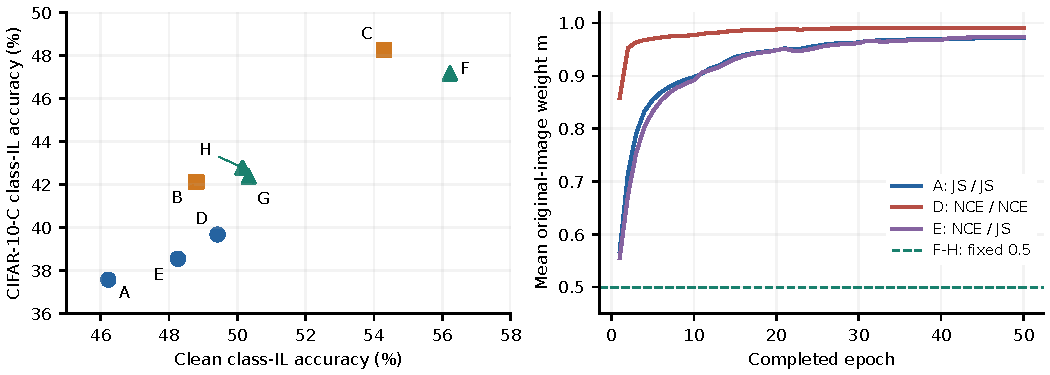
\includegraphics[width=\textwidth]{figures/overview.pdf}
\caption{\textbf{Performance and mixture diagnostics.} Left: clean versus
corrupted class-IL accuracy; labels identify the runs in Table~\ref{tab:main}.
Right: recorded epoch means of the original-image weight for the three guided
mixers, with the chain-aware fixed value shown for reference. High $m$ weakens
the transformed contribution. These diagnostics characterize our implementation,
not verified MetaMix author code.}
\label{fig:overview}
\end{figure*}

\section{Adaptive Chain Mixing}
\subsection{Problem Formulation}
Let $\mathcal{D}_1,\ldots,\mathcal{D}_T$ be successive training-task
distributions. At task $t$, the learner accesses current examples and a bounded
replay memory, but not earlier full datasets. Let $\mathcal{Q}$ denote a target
distribution over corruption transformations unavailable to the training
procedure. The desired final-model performance can be expressed as
\begin{equation}
\mathcal{R}_{\mathcal{Q}}(\theta_T)=
\frac{1}{T}\sum_{t=1}^{T}
\mathbb{E}_{(x,y)\sim\mathcal{D}_t,\,c\sim\mathcal{Q}}
[\CE(f_{\theta_T}(c(x)),y)].
\label{eq:target}
\end{equation}
This expresses the generalization goal, not an optimized training loss;
we report test accuracy rather than estimating this cross-entropy risk.
Training observes neither samples from $\mathcal{Q}$ nor its gradients.
Clean accuracy and retention across the accumulated classes remain relevant.

\paragraph{Finite augmentation candidates.}
Let $\mathcal{O}$ contain $M$ operations and let chains have maximum depth $D$.
Allowing ordered choices with repetition gives
\begin{equation}
|\mathcal{A}_{\leq D}|=\sum_{d=1}^{D}M^d
\label{eq:space}
\end{equation}
operator sequences before accounting for severity and other parameters.
This counts sequences, not necessarily distinct transformed images. The
expression motivates sampling as the space grows; it is not a measured runtime
bound or evidence that every sequence must be visited for robust learning.

At a training step, we draw $K$ candidate chains per image and view from an
augmentation sampling distribution $q$, with $K=3$ in our experiments.
The mixer maps their effects and learner context to simplex weights
$w_\phi\in\Delta^{K-1}$. It learns their combination while $q$ remains fixed
by the stochastic augmentation procedure. Our hypothesis is that these
conditional weights can yield more useful representation-learning views than
weights that ignore candidate effects. The controlled test would hold strength,
view-sharing, and compute conventions fixed; our current experiments only
partially isolate this comparison.

Following a MetaMix-inspired setup, separate pseudo-seen and pseudo-unseen
operation pools support classifier and mixer updates. Consistency on the
latter is a surrogate for adaptation, not access to $\mathcal{Q}$ or a guarantee
of transfer. The classifier and mixer are trained alternately as specified
below. At test time, only the classifier is used; the mixer supports robustness
through training rather than choosing transformations for test inputs.

\subsection{Classifier and Replay Objective}
Let $f_\theta(x)\in\mathbb{R}^{10}$ be classifier logits and
$h_\theta(x)\in\mathbb{R}^{128}$ the pooled feature. A current batch $B_t$
and a replay batch $B_r$ form an augmentation batch $A=B_t\cup B_r$.
A separate replay sample $B_z$ contains stored logits $z^{\mathrm{old}}$.
We write $\langle\cdot\rangle_B$ for a batch mean and use
\begin{align}
\mathcal{L}_{\mathrm{base}}(\theta)
={}&\langle\CE(f_\theta(x),y)\rangle_{B_t}\nonumber\\
&+0.5\langle\CE(f_\theta(x),y)\rangle_{B_r}\nonumber\\
&+0.2\langle\operatorname{MSE}(f_\theta(x),z^{\mathrm{old}})\rangle_{B_z}.
\label{eq:base}
\end{align}
MSE averages over examples and the ten logit coordinates. Missing replay
terms are zero. Stored current-example logits are captured before the
classifier update. The reservoir stores raw images, labels, and these logits;
only current examples are inserted. Its insertion counter advances for every
presentation, including repeated presentations over epochs, so it samples
the presentation stream rather than a set of unique images.

\subsection{Image Mixtures and Operation Splits}
For image $x_i$, view $v\in\{1,2\}$, and three candidate chains
$a_{ivk}$, the mixed input is
\begin{equation}
\widetilde{x}_{iv}=m_{iv}x_i+(1-m_{iv})
\sum_{k=1}^{3} w_{ivk}a_{ivk}(x_i),\qquad \sum_k w_{ivk}=1.
\label{eq:mix}
\end{equation}
Each batch splits nine licensed AugMix operations into disjoint pools of
5--7 pseudo-seen and 2--4 pseudo-unseen operations. Two sets of three chains
are sampled from each pool. A chain applies 1--3 operations at severity 3.
Pseudo-seen mixtures train the classifier; pseudo-unseen mixtures train the
controller. The split is resampled every batch: ``unseen'' is a within-batch
designation, not a held-out test distribution. CIFAR-10-C test images never
enter either training pool.

Random controls draw $m\sim\operatorname{Beta}(1,1)$ and
$w\sim\operatorname{Dirichlet}(1,1,1)$ independently per image and view.
The MetaMix-guided controller instead produces one $m$ and one vector $w$
per image, shared across its two views. We preserve this distinction rather
than presenting the random/learned comparison as a pure one-factor ablation.

\subsection{Separate Objectives for Representation and Mixing}
We write $\mathcal{C}_{\mathrm{cls}}$ for classifier consistency and
$\mathcal{C}_{\mathrm{mix}}$ for the mixer's surrogate. Each can independently
be JS or class-aware InfoNCE. The former changes the classifier's parameters;
the latter changes the weights assigned to candidate chains. Our focal
configuration uses feature InfoNCE for the classifier and prediction JS for
the mixer. This is an empirical design choice, not a claim that JS measures
unseen robustness directly.

\paragraph{Prediction-space JS.}
For predictions $p_{iv}=\operatorname{softmax}(f_\theta(x_{iv}))$, with
$x_{i0}=x_i$ and $x_{iv}=\widetilde{x}_{iv}$ for $v>0$, let
$\bar p_i=(p_{i0}+p_{i1}+p_{i2})/3$. We use
\begin{equation}
\JS=\frac{1}{3N}\sum_{i=1}^{N}\sum_{v=0}^{2}
\KL(p_{iv}\Vert\bar p_i).
\label{eq:js}
\end{equation}
The implementation clamps the mean probability before taking its logarithm.

\paragraph{Class-aware feature InfoNCE.}
Normalize pooled features to unit length and index all $3N$ views by $a$.
Let $\mathcal{P}(a)$ contain the two other views of the same batch entry.
The allowed denominator set is
\begin{equation}
\mathcal{D}(a)=\mathcal{P}(a)\cup\{b:y_b\ne y_a\}.
\end{equation}
With $u_a$ the normalized feature and temperature $\tau=0.1$,
\begin{equation}
\NCE=-\frac{1}{3N}\sum_{a=1}^{3N}\frac{1}{2}
\sum_{p\in\mathcal{P}(a)}
\log\frac{\exp(u_a^\top u_p/\tau)}
{\sum_{b\in\mathcal{D}(a)}\exp(u_a^\top u_b/\tau)}.
\label{eq:nce}
\end{equation}
The anchor is excluded. Same-class nonpositive entries are also excluded.
No projection head, reconstruction decoder, or augmented-view CE is used in
these eight runs. Both objectives include current and replay-CE examples.

\subsection{Alternating Updates and Their Gradient Meaning}
The classifier receives one SGD update using
\begin{equation}
\mathcal{L}_{\mathrm{cls}}=\mathcal{L}_{\mathrm{base}}+
\mathcal{C}_{\mathrm{cls}}^{\mathrm{seen}},\quad
\mathcal{C}_{\mathrm{cls}}\in\{\JS,\NCE\}.
\end{equation}
Mixture weights are detached during this update. Next, the updated classifier
$\theta^+$ is held fixed while three controller SGD steps minimize
\begin{equation}
\mathcal{L}_{\mathrm{mix}}(\phi)=
\langle\CE(f_{\theta^+}(x),y)\rangle_A+
\mathcal{C}_{\mathrm{mix}}^{\mathrm{unseen}}(\theta^+,\phi).
\label{eq:outer}
\end{equation}
Context and original-view outputs are detached. The original CE term is
reported but has zero gradient with respect to $\phi$. Mixer gradients pass
through the blended augmented images and the frozen classifier. There is
\emph{no differentiation through the classifier optimization step} and no
explicit post-update replay-retention term. Although the code groups this
procedure under a bi-level trainer, the implemented gradient is an alternating
fixed-classifier partial derivative, not an unrolled bilevel hypergradient.
Its equivalence to the original MetaMix solver has not been established.

This distinction matters. For JS and deterministic evaluation, setting
$m=1$ makes all views identical, giving zero consistency loss irrespective of
the candidate chains. Thus the objective admits an identity-mixture solution.
This is an available solution, not a proof that optimization must reach it.
InfoNCE retains cross-image comparisons and need not vanish at identity;
high learned $m$ in that setting is an empirical observation rather than the
same zero-loss argument.

\subsection{Conditioning Weights on the Sampled Chains}
The temporal controller uses an LSTM cell of hidden size five. Its detached
258-dimensional input concatenates the batch-level dot product between clean
current and replay CE gradients, replay CE, a 128-dimensional replay feature,
and a 128-dimensional current feature. Scalars are broadcast; feature pairs
are assigned cyclically when batch sizes differ. Empty replay supplies zeros
for the replay-related context. These choices are explicit implementation
conventions.

Hidden and cell states use 64 persistent batch-position slots: 32 current and
32 replay. They are not image identities. Inactive slots are retained and state
is detached across batches. The transition computed before controller
optimization is committed once; all three mixer steps reuse the incoming state.

The baseline guided controller has no candidate-chain input. Our chain-aware
extension computes a descriptor for each candidate:
\begin{equation}
d_{ivk}=\sg\!\left[
\begin{array}{c}
h_\theta(a_{ivk}(x_i))-h_\theta(x_i)\\
p_\theta(a_{ivk}(x_i))-p_\theta(x_i)
\end{array}\right]\in\mathbb{R}^{138}.
\end{equation}
Concatenating $d_{ivk}$ with the five-dimensional LSTM hidden state yields
143 inputs to a shared linear--ReLU--linear scorer (143--32--1).
Writing $s_i$ for the temporal hidden state and $g_\phi$ for the scorer,
\begin{equation}
w_{ivk}=\frac{\exp g_\phi([s_i;d_{ivk}])}
{\sum_{j=1}^{3}\exp g_\phi([s_i;d_{ivj}])}.
\label{eq:weights}
\end{equation}
Thus weights respond to the sampled chains separately for each image and view.
The operations, chain depths, and candidate sampling remain stochastic and are
not optimized by the mixer. The final scorer layer is initialized to zero, yielding uniform initial
weights. We fix $m_{iv}=0.5$, so augmentation retains a nonzero contribution.
Seen descriptors use the classifier before its update; unseen descriptors
use the updated classifier and remain fixed during the three mixer steps.
This extension simultaneously changes candidate conditioning, per-view
weighting, and the treatment of $m$; their separate effects are not identified.

\begin{table*}[t]
\centering\small
\setlength{\tabcolsep}{7pt}
\begin{tabular}{lllrrrr}
\toprule
ID & Mixer & Classifier / mixer & Clean class-IL & Corrupt class-IL & Clean task-IL & Corrupt task-IL \\
\midrule
A & Guided & JS / JS & 46.22 & 37.58 & 89.17 & 83.33 \\
B & Random & JS / none & 48.80 & 42.11 & 89.71 & 85.41 \\
C & Random & NCE / none & \underline{54.30} & \textbf{48.27} & \textbf{91.20} & \textbf{87.19} \\
D & Guided & NCE / NCE & 49.42 & 39.68 & 90.08 & 83.24 \\
E & Guided & NCE / JS & 48.26 & 38.55 & 89.25 & 82.69 \\
\rowcolor{ourrow} F & Chain-aware & NCE / JS & \textbf{56.22} & \underline{47.17} & \underline{91.02} & \underline{86.24} \\
G & Chain-aware & JS / JS & 50.33 & 42.37 & 90.50 & 85.66 \\
H & Chain-aware & NCE / NCE & 50.15 & 42.79 & 90.99 & 86.01 \\
\bottomrule
\end{tabular}
\caption{\textbf{All completed core experiments.} Accuracy (\%), seed 17.
Guided denotes our MetaMix-guided implementation, not verified author code.
NCE denotes class-aware InfoNCE. All chain-aware runs fix $m=0.5$; all rows use
CE + DER++. Corrupt scores average all 15 corruptions and five severities.
Blue highlights our focal chain-aware InfoNCE/JS configuration.
Bold marks the best score and underlining the second-best, ranked using unrounded values per column.}
\label{tab:main}
\end{table*}


\section{Experimental Protocol}
\paragraph{Data and budgets.}
We use CIFAR-10~\cite{krizhevsky2009learning} with five sequential class pairs:
$(0,1),(2,3),(4,5),(6,7),(8,9)$. All 50,000 training images are used, with
10 epochs for each task, batch size 32, replay size up to 32, and reservoir
capacity 500. Each run has 15,650 classifier updates and 500,000 current-image
presentations. All use seed 17. Learned mixers have three controller updates
per classifier step, whereas random controls have none; equal classifier
budgets therefore do not imply equal compute budgets.

\paragraph{Model and optimization.}
The classifier has six $3\times3$ convolutions, two each at widths 32, 64, and
128, with BatchNorm and ReLU. Average pooling follows the first two stages;
global average pooling gives 128 features and a linear ten-class head.
It contains 288,746 parameters, excluding the controller. Images remain
$32\times32$, normalized by means $(0.4914,0.4822,0.4465)$ and standard
deviations $(0.2470,0.2435,0.2616)$. We use classifier SGD at 0.03 and mixer
SGD at 0.05, with no momentum, weight decay, or learning-rate schedule.
All consistency coefficients are one. Experiments run in CUDA float32 on
an RTX 3060 Ti. No extra crop, flip, pretraining, or test-time augmentation
is used.

\paragraph{BatchNorm and sampling controls.}
The original and two seen views use one joint training-mode forward, followed
by a separate stored-logit replay forward when replay is available. Context
forwards use cloned buffers; descriptor and outer forwards use evaluation
mode without committing BatchNorm changes. Random controls still generate
pseudo-unseen chains to preserve operation-RNG consumption. Sampling hashes
match at every update for four runs: random JS, random InfoNCE, guided
InfoNCE/InfoNCE, and guided InfoNCE/JS. The guided JS reference predates this
logging, and we do not extend the fingerprint claim to the chain-aware runs.

\paragraph{Evaluation.}
We evaluate the final checkpoint on 10,000 clean test images and all 15
CIFAR-10-C corruptions at five severities, totaling 750,000 corrupted
predictions. Class-IL predicts among all ten classes; task-IL is given the
correct two-class pair. Neither test-time augmentation nor test-based
checkpoint selection is used. Category scores average corruption accuracies,
each already averaged over five severities. Overall accuracy is
\begin{equation}
A_{\mathrm{all}}=\frac{3A_{\mathrm{noise}}+4A_{\mathrm{blur}}+
4A_{\mathrm{weather}}+4A_{\mathrm{digital}}}{15}.
\end{equation}
This is accuracy, not a normalized corruption-error score. All corruptions
contain the same balanced labels, so overall task-IL accuracy also equals
an equally weighted average across the five tasks. Separate per-task
trajectories and backward-transfer measurements are not available in these
evaluation artifacts.



\begin{table*}[t]
\centering\small
\begin{tabular}{lllrrrrr}
\toprule
\multicolumn{8}{l}{\textbf{Class-IL}} \\
ID & Mixer & Objectives & Noise & Blur & Weather & Digital & Overall \\
\midrule
A & Guided & JS / JS & 32.75 & 39.33 & 38.63 & 38.40 & 37.58 \\
B & Random & JS / none & 40.38 & 44.00 & 41.69 & 41.95 & 42.11 \\
C & Random & NCE / none & \textbf{48.78} & \textbf{49.96} & \underline{47.48} & \underline{46.98} & \textbf{48.27} \\
D & Guided & NCE / NCE & 36.42 & 40.35 & 40.54 & 40.59 & 39.68 \\
E & Guided & NCE / JS & 34.71 & 40.06 & 39.16 & 39.31 & 38.55 \\
\rowcolor{ourrow} F & Chain-aware & NCE / JS & \underline{45.06} & \underline{47.26} & \textbf{47.51} & \textbf{48.31} & \underline{47.17} \\
G & Chain-aware & JS / JS & 36.79 & 45.67 & 42.39 & 43.25 & 42.37 \\
H & Chain-aware & NCE / NCE & 39.84 & 44.79 & 42.53 & 43.26 & 42.79 \\
\midrule
\multicolumn{8}{l}{\textbf{Task-IL}} \\
ID & Mixer & Objectives & Noise & Blur & Weather & Digital & Overall \\
\midrule
A & Guided & JS / JS & 81.11 & 82.76 & 85.06 & 83.85 & 83.33 \\
B & Random & JS / none & 83.22 & 85.60 & 86.44 & 85.84 & 85.41 \\
C & Random & NCE / none & \textbf{86.23} & \textbf{87.03} & \textbf{88.23} & \textbf{87.03} & \textbf{87.19} \\
D & Guided & NCE / NCE & 81.53 & 82.69 & 84.75 & 83.57 & 83.24 \\
E & Guided & NCE / JS & 79.01 & 82.57 & 84.74 & 83.52 & 82.69 \\
\rowcolor{ourrow} F & Chain-aware & NCE / JS & \underline{85.79} & 85.46 & \underline{87.50} & 86.11 & \underline{86.24} \\
G & Chain-aware & JS / JS & 82.96 & \underline{85.78} & 86.92 & \underline{86.30} & 85.66 \\
H & Chain-aware & NCE / NCE & 84.69 & 85.54 & 87.42 & 86.04 & 86.01 \\
\bottomrule
\end{tabular}
\caption{\textbf{Corruption-category accuracy (\%).} Each category averages
five-severity corruption means. Overall weights Noise, Blur, Weather, and
Digital by 3, 4, 4, and 4 corruptions, respectively. NCE is class-aware InfoNCE;
all chain-aware runs fix $m=0.5$. Blue highlights chain-aware InfoNCE/JS;
bold marks the best score and underlining the second-best, ranked using unrounded values per column.}
\label{tab:categories}
\end{table*}


\section{Results}
\paragraph{Main result: adapting the sampled chain mixtures.}
\textbf{Chain-aware InfoNCE/JS achieves the best clean class-IL accuracy
(56.22\%) and the second-best overall corrupted class-IL accuracy (47.17\%).}
Against guided InfoNCE/JS, the configuration gains 7.96 clean and 8.62 corrupted
percentage points. It also leads class-IL Weather (47.51\%) and Digital
(48.31\%). We highlight this configuration in blue in the result tables.
The gains apply to the combined controller changes, not chain conditioning
alone; random InfoNCE remains stronger on overall corrupted accuracy.

\subsection{Evidence for the Finite-Candidate Hypothesis}
Table~\ref{tab:main} reports all eight runs using three candidate chains per
view. The gain over the guided mixer is consistent with the hypothesis, but
does not isolate candidate conditioning. Random InfoNCE reaches 48.27\%
corrupted class-IL, the best observed result. It exceeds guided
InfoNCE/InfoNCE by 8.59 percentage points and random JS by 6.15 points.
Random JS also exceeds guided JS by 4.53 points. Thus learned mixing is not
uniformly beneficial in this implementation, and replacing JS with class-aware
InfoNCE is particularly effective under the random controller.

The random/learned contrast has qualifications: weights are independent across
views only in the random case, and the guided controller incurs additional
optimization. Consequently, these results compare complete configurations
rather than identifying the isolated causal effect of learning the weights.

\subsection{The Two Objectives Should Be Tested Separately}
Keeping the guided controller and classifier InfoNCE fixed, changing its
mixer objective from InfoNCE to JS reduces clean class-IL from 49.42\% to
48.26\% and corrupted class-IL from 39.68\% to 38.55\%. This objective-only
change does not rescue the original guided controller at this seed.

Within the chain-aware architecture, the pattern differs. InfoNCE/JS gives
56.22\% clean and 47.17\% corrupted class-IL. Changing only classifier
consistency to JS reduces these to 50.33\% and 42.37\%, drops of 5.89 and
4.80 points. Keeping classifier InfoNCE but changing the mixer objective to
InfoNCE yields 50.15\% and 42.79\%, drops of 6.07 and 4.38 points.
Using the same objective for both components is therefore not the best
observed choice for this controller.

This does not establish a universal preference for JS as a mixer objective:
the guided-controller ablation shows the opposite local ranking. Instead,
the evidence points to an interaction between the controller parameterization
and the objective. Classifier feature learning and candidate-mixture selection
should be evaluated as separate design decisions.

\subsection{Clean and Corrupted Rankings Differ}
Chain-aware InfoNCE/JS has the highest clean class-IL, 1.92 points above
random InfoNCE, but its corrupted class-IL is 1.10 points lower.
Random InfoNCE also has the highest task-IL scores, 91.20\% clean and
87.19\% corrupted. The chain-aware gain on clean class-IL therefore does
not imply dominance across metrics.

The within-chain-aware gaps are much smaller in task-IL: corrupted accuracy
is 86.24\% for InfoNCE/JS, 85.66\% for JS/JS, and 86.01\% for
InfoNCE/InfoNCE. Supplying the task identity changes the observable difficulty
and ranking gaps. The aggregates are consistent with sensitivity to the
all-class decision problem, but do not identify a specific calibration or
cross-task-confusion mechanism without per-task and confusion-matrix analysis.

\subsection{Category-Level Behavior}
Table~\ref{tab:categories} shows the breakdown by corruption family. Random
InfoNCE leads class-IL Noise and Blur, while chain-aware InfoNCE/JS leads
Weather and Digital. For the chain-aware JS/JS run, Noise class-IL falls to
36.79\%, compared with 45.06\% for InfoNCE/JS. The InfoNCE/InfoNCE mixer
recovers some Noise performance (39.84\%) but remains below InfoNCE/JS
in every class-IL category.

The task-IL comparison is less uniform. Chain-aware JS/JS has slightly higher
Blur and Digital accuracy than chain-aware InfoNCE/JS (85.78\% versus
85.46\%, and 86.30\% versus 86.11\%), despite lower overall accuracy.
These differences are descriptive single-seed observations, not statistical
significance claims. Appendix~\ref{sec:appendix} gives all per-corruption means.

\subsection{Mixture Strength and an Objective Shortcut}
Figure~\ref{fig:overview} shows that the guided controllers increasingly favor
the original image. Final-epoch mean $m$ is 0.9726 for guided JS/JS,
0.9916 for guided InfoNCE/InfoNCE, and 0.9739 for guided InfoNCE/JS.
For the latter run, 99.26\% of recorded final-epoch values exceed 0.95.
This substantially reduces the contribution of transformed chains.

Fixing $m=0.5$ removes this particular strength shortcut, but does not guarantee
useful mixtures: a controller can still favor relatively mild candidate
chains. The chain-aware descriptors allow content-dependent scoring, and the
shared scorer is equivariant to candidate reordering. However, our results
do not separate the value of descriptors from fixing $m$ or learning
independent per-view weights. The negative chain-aware objective ablations
also show that avoiding $m\approx1$ is not sufficient for the best accuracy.

\section{Limitations and Reproducibility}
\paragraph{Statistical and selection limits.}
All reported runs use one seed and one dataset/task order. We cannot estimate
training-seed variability, report confidence intervals for method differences,
or claim statistical superiority. The 750,000 corrupted predictions are
repeated transformations of 10,000 test images, not 750,000 independent
training replications. Later experiment choices were informed by earlier
test results, so the sequence has exploratory selection bias even though
checkpoints were not selected using test accuracy. Confirmation requires
fresh seeds and a validation-driven design protocol.

\paragraph{Mechanistic limits.}
The chain-aware extension couples fixed mixture strength, candidate descriptors,
and per-view weights. A fixed-$m$ random control, a fixed-$m$ controller without
candidate descriptors, and matched shared-versus-independent-view weights
are needed to attribute the gain. The JS/class-aware InfoNCE replacements
also differ in numerical scale; coefficient and temperature sweeps would be
needed before calling the negative results an intrinsic failure of an objective.
No unaugmented DER++ baseline is included in this eight-run comparison.

\paragraph{Fidelity and compute limits.}
The original authors' autograd semantics have not been verified. Our frozen
updated-classifier gradient should not be advertised as their exact solver.
Our model, budget, and state/BatchNorm conventions also limit comparisons with
published benchmarks. Equal numbers of classifier steps do not control for
candidate descriptor forwards or mixer optimization cost. We have not measured
a standardized compute--accuracy trade-off. The finite-candidate motivation
is not a demonstrated efficiency gain: we do not vary $K$, compare against
exhaustive enumeration, or show that adaptive mixing requires fewer candidates
for a target accuracy. Descriptor evaluation and mixer updates add work beyond
the random baseline.

\paragraph{Reproducibility artifacts.}
Every reported run has a completion record, full evaluation, configuration,
epoch summary, and source snapshot checked against SHA256 hashes. Epoch-boundary
checkpoints preserve classifier and controller weights, optimizer states,
reservoir contents, recurrent state, and random-number generators. Tests check
objective formulas, same-class exclusion, finite mixer gradients, detached
classifier gradients, BatchNorm behavior, and exact next-step resume.
These software checks do not establish statistical superiority. Auxiliary
reconstruction and multi-head experiments are outside this comparison.

\section{Conclusion}
The combinatorial augmentation space motivates learning from finite stochastic
candidate sets. We hypothesize that adapting how these candidates are combined
can improve the training views used for corruption-robust representation
learning. Our chain-aware mixer weights sampled AugMix chains using their
effects on the classifier and temporal learner context, with separate objectives
for representation learning and mixer adaptation. Chain-aware InfoNCE/JS
achieves 56.22\% clean and 47.17\% corrupted class-IL accuracy, improving on
the guided configuration and the matching-objective chain-aware variants.
Random InfoNCE remains strongest on overall corrupted accuracy. These results
motivate further tests of the hypothesis without establishing superiority of
adaptive mixing or computational efficiency. Matched controller ablations,
candidate-budget sweeps, and fresh seeds are needed to determine when learning
to combine sampled chains improves unseen-corruption generalization.

{\small
\bibliographystyle{ieeenat_fullname}
\bibliography{references}
}

\clearpage
\onecolumn
\appendix
\section{Per-Corruption Results and Reproduction}
\label{sec:appendix}
The following tables report all eight runs for each corruption, averaged over
five severities. Every cell is accuracy in percent; bold marks the best
and underlining the second-best score, ranked before rounding within each column. The same clean test labels are used at each
severity. The category weights in the main text are essential: averaging the
four category means without weights would overrepresent Noise.

Run IDs match Table~\ref{tab:main}. The artifacts are organized under
\texttt{results/corrected\_mixing\_seed17/}. The script
\texttt{scripts/summarize\_corruption\_categories.py} validates complete
evaluation counts and regenerates the repository reports. The accompanying
\texttt{generate\_assets.py} generates this paper's tables and figure from
those committed artifacts, rather than manually transcribing the results.

For example, the chain-aware InfoNCE/InfoNCE configuration is
\texttt{configs/chain\_aware\_infonce\_infonce.json}; it can be launched with
\texttt{scripts/run\_experiment.py}, supplying the configuration,
\texttt{--data-root}, and \texttt{--run}. CUDA and the verified clean/corrupted
datasets are required. Output directories must be fresh or contain an exact
matching configuration/source checkpoint. Data, checkpoint weights, and full
batch traces are not included in the committed result archive.

\begin{center}
\begin{minipage}{\textwidth}
\centering\small
\setlength{\tabcolsep}{6pt}
\begin{tabular}{lllrrrrrr}
\toprule
 &  &  & \multicolumn{3}{c}{Class-IL} & \multicolumn{3}{c}{Task-IL} \\
ID & Mixer & Objectives & Gauss & Shot & Impulse & Gauss & Shot & Impulse \\
\midrule
A & Guided & JS / JS & 34.12 & 35.89 & 28.25 & 81.52 & 83.01 & 78.81 \\
B & Random & JS / none & 40.77 & 42.54 & 37.83 & 83.13 & 84.93 & 81.60 \\
C & Random & NCE / none & \textbf{48.50} & \textbf{50.78} & \textbf{47.06} & \textbf{86.16} & \textbf{87.54} & \textbf{85.00} \\
D & Guided & NCE / NCE & 37.25 & 39.50 & 32.51 & 81.41 & 83.45 & 79.73 \\
E & Guided & NCE / JS & 35.03 & 37.73 & 31.38 & 78.43 & 81.49 & 77.11 \\
\rowcolor{ourrow} F & Chain-aware & NCE / JS & \underline{45.16} & \underline{47.92} & \underline{42.08} & \underline{85.58} & \underline{87.19} & \underline{84.60} \\
G & Chain-aware & JS / JS & 37.75 & 39.82 & 32.79 & 83.11 & 84.97 & 80.79 \\
H & Chain-aware & NCE / NCE & 41.11 & 42.84 & 35.57 & 84.83 & 86.12 & 83.14 \\
\bottomrule
\end{tabular}
\captionof{table}{Noise corruptions: accuracy (\%) averaged over five severities. Bold: best; underlined: second-best (unrounded ranks).}
\end{minipage}
\end{center}
\begin{center}
\begin{minipage}{\textwidth}
\centering\small
\setlength{\tabcolsep}{6pt}
\begin{tabular}{lllrrrrrrrr}
\toprule
 &  &  & \multicolumn{4}{c}{Class-IL} & \multicolumn{4}{c}{Task-IL} \\
ID & Mixer & Objectives & Defocus & Glass & Motion & Zoom & Defocus & Glass & Motion & Zoom \\
\midrule
A & Guided & JS / JS & 43.32 & 35.15 & 36.27 & 42.58 & 85.67 & 77.14 & 83.40 & 84.82 \\
B & Random & JS / none & 47.97 & 38.16 & 42.82 & 47.05 & \underline{88.88} & 79.21 & 86.49 & 87.83 \\
C & Random & NCE / none & \textbf{53.12} & \textbf{44.62} & \textbf{49.18} & \textbf{52.92} & \textbf{89.74} & \textbf{82.44} & \textbf{87.04} & \textbf{88.90} \\
D & Guided & NCE / NCE & 44.93 & 35.86 & 37.25 & 43.34 & 86.75 & 76.52 & 82.54 & 84.96 \\
E & Guided & NCE / JS & 44.12 & 34.97 & 37.67 & 43.48 & 85.85 & 77.53 & 82.29 & 84.61 \\
\rowcolor{ourrow} F & Chain-aware & NCE / JS & \underline{52.44} & \underline{40.98} & 45.35 & \underline{50.27} & 88.35 & \underline{80.99} & 85.39 & 87.10 \\
G & Chain-aware & JS / JS & 50.77 & 36.39 & \underline{45.93} & 49.59 & 88.88 & 79.55 & \underline{86.79} & \underline{87.89} \\
H & Chain-aware & NCE / NCE & 48.95 & 38.01 & 43.66 & 48.52 & 88.40 & 80.49 & 85.74 & 87.54 \\
\bottomrule
\end{tabular}
\captionof{table}{Blur corruptions: accuracy (\%) averaged over five severities. Bold: best; underlined: second-best (unrounded ranks).}
\end{minipage}
\end{center}
\clearpage
\begin{center}
\begin{minipage}{\textwidth}
\centering\small
\setlength{\tabcolsep}{6pt}
\begin{tabular}{lllrrrrrrrr}
\toprule
 &  &  & \multicolumn{4}{c}{Class-IL} & \multicolumn{4}{c}{Task-IL} \\
ID & Mixer & Objectives & Snow & Frost & Fog & Bright & Snow & Frost & Fog & Bright \\
\midrule
A & Guided & JS / JS & 37.64 & 34.71 & 38.53 & 43.62 & 83.73 & 83.62 & 84.82 & 88.09 \\
B & Random & JS / none & 41.02 & 37.45 & 42.09 & 46.21 & 85.08 & 85.03 & 86.48 & 89.18 \\
C & Random & NCE / none & \underline{46.84} & \textbf{43.52} & \underline{48.42} & \underline{51.13} & \textbf{87.39} & \textbf{87.00} & \textbf{87.96} & \textbf{90.58} \\
D & Guided & NCE / NCE & 40.22 & 36.49 & 39.48 & 45.98 & 84.66 & 82.86 & 83.22 & 88.26 \\
E & Guided & NCE / JS & 38.25 & 34.89 & 40.20 & 43.28 & 83.21 & 82.99 & 84.71 & 88.06 \\
\rowcolor{ourrow} F & Chain-aware & NCE / JS & \textbf{47.50} & \underline{42.61} & \textbf{48.49} & \textbf{51.44} & 86.67 & \underline{86.35} & 86.87 & \underline{90.10} \\
G & Chain-aware & JS / JS & 39.77 & 37.84 & 44.17 & 47.76 & 85.32 & 85.75 & 86.98 & 89.63 \\
H & Chain-aware & NCE / NCE & 41.20 & 38.63 & 44.44 & 45.85 & \underline{86.70} & 86.14 & \underline{87.06} & 89.77 \\
\bottomrule
\end{tabular}
\captionof{table}{Weather corruptions: accuracy (\%) averaged over five severities. Bold: best; underlined: second-best (unrounded ranks).}
\end{minipage}
\end{center}
\begin{center}
\begin{minipage}{\textwidth}
\centering\small
\setlength{\tabcolsep}{6pt}
\begin{tabular}{lllrrrrrrrr}
\toprule
 &  &  & \multicolumn{4}{c}{Class-IL} & \multicolumn{4}{c}{Task-IL} \\
ID & Mixer & Objectives & Contrast & Elastic & Pixel & JPEG & Contrast & Elastic & Pixel & JPEG \\
\midrule
A & Guided & JS / JS & 31.78 & 42.22 & 36.46 & 43.13 & 76.38 & 85.66 & 86.27 & 87.08 \\
B & Random & JS / none & 36.30 & 45.94 & 39.71 & 45.83 & 80.73 & 87.56 & 87.10 & 87.98 \\
C & Random & NCE / none & \textbf{39.44} & \textbf{50.80} & \underline{46.85} & \underline{50.85} & \underline{80.94} & \textbf{88.42} & \textbf{89.19} & \textbf{89.59} \\
D & Guided & NCE / NCE & 31.83 & 44.81 & 40.23 & 45.50 & 72.64 & 86.62 & 87.01 & 88.02 \\
E & Guided & NCE / JS & 31.98 & 43.82 & 37.23 & 44.22 & 76.47 & 85.68 & 85.33 & 86.60 \\
\rowcolor{ourrow} F & Chain-aware & NCE / JS & \underline{38.75} & \underline{50.65} & \textbf{51.21} & \textbf{52.62} & 79.25 & 87.43 & \underline{88.96} & 88.79 \\
G & Chain-aware & JS / JS & 37.94 & 48.22 & 39.21 & 47.62 & \textbf{81.13} & \underline{87.84} & 87.47 & 88.77 \\
H & Chain-aware & NCE / NCE & 35.55 & 47.34 & 42.63 & 47.54 & 79.45 & 87.77 & 88.13 & \underline{88.82} \\
\bottomrule
\end{tabular}
\captionof{table}{Digital corruptions: accuracy (\%) averaged over five severities. Bold: best; underlined: second-best (unrounded ranks).}
\end{minipage}
\end{center}

\end{document}
